\section{Experimental validation of regime-dependent behavior}
\label{sec:experiments}

This section empirically validates the regime-dependent framework by systematically traversing operating points across capacity, bandwidth, and coordination dimensions, focusing on qualitative regime transitions rather than absolute performance gains.


\subsection{Experimental methodology and regime probing strategy}

\begin{figure}[t]
\centering
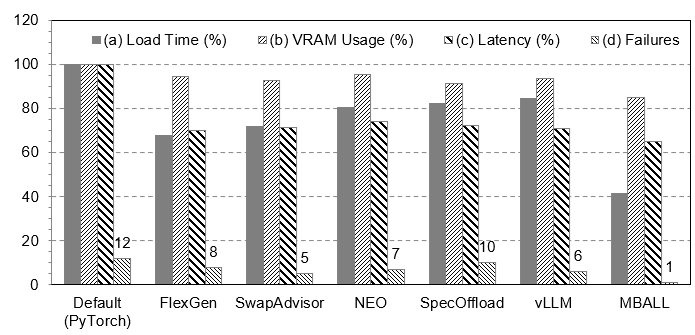
\includegraphics[width=0.95\linewidth]{figures/mball_consolidated.png}
\caption{\textbf{Regime-oriented experimental probes across baselines.} Consolidated results summarizing (a) model loading time, (b) memory efficiency, (c) inference latency, and (d) stability outcomes across representative orchestration baselines. The figure illustrates that improvements are regime-dependent and can invert or collapse when operating points cross regime boundaries.}
\label{fig:consolidated}
\end{figure}

Figure~\ref{fig:consolidated} provides an overview of the regime-oriented probes and baseline outcomes used throughout this section. To validate the regime-dependent principles derived in Sections~\ref{sec:regime} and \ref{sec:model}, we design experiments that explicitly probe transitions between operational regimes rather than optimizing for peak performance under a single configuration. Our methodology focuses on controlled variation of system capacity and sustained cross-tier transfer bandwidth to move inference workloads across analytically identified regime boundaries.

Instead of treating system parameters as fixed, we systematically vary (i) the ratio between fast and intermediate memory capacity and (ii) the sustained bandwidth available for cross-tier data transfer. These variations shift the system\textquotesingle s operating point in the regime space, enabling direct observation of changes in dominant latency components. Metrics are selected to reflect regime behavior---such as changes in latency decomposition, stability, and sensitivity to orchestration---rather than raw throughput alone.


\subsection{Observing regime transitions in real AI inference systems}
\textbf{Capacity-limited regimes.}
We first examine configurations in which fast-memory capacity is insufficient to accommodate the working set required for effective locality. In this capacity-limited regime, increasing orchestration depth does not substantially alter execution behavior. Instead, latency is dominated by frequent eviction and reloading, and memory access costs grow sharply as working-set pressure increases. Empirically, inference latency becomes highly sensitive to small changes in working-set size or batch configuration, while remaining largely insensitive to coordination strategies.

\textbf{Coordination-dominated regimes.}
When fast and intermediate memory together can absorb most of the working set, the system enters a coordination-dominated regime. In this regime, computation, memory access, transfer, and synchronization costs are of comparable magnitude, creating opportunities for orchestration to reshape end-to-end behavior. We observe that within this regime, changes in orchestration strategy produce measurable shifts in latency composition (rather than uniform scaling), consistent with the model in Eq.~\ref{eq:latency_decomp}.

\textbf{I/O-limited regimes.}
Finally, we evaluate configurations in which cross-tier data transfer approaches sustained bandwidth limits. In this I/O-limited regime, transfer costs dominate execution regardless of coordination strategy. Once transfer demand saturates available bandwidth, latency scales directly with data movement volume and coordination overhead becomes additive rather than compensatory.

\subsection{Quantitative evidence of abrupt regime transitions}

A central claim of this work is that regime transitions are \emph{abrupt}
rather than gradual.
To quantify this, we measure the \emph{sharpness coefficient}
$S = |d\ln T_{\mathrm{total}} / d\ln R|$, which captures the fractional
change in total latency per fractional change in the control parameter
$R \in \{R_C, R_B\}$.
A transition is defined as abrupt if $S > S^* = 2.0$, i.e., a 10\% change
in $R$ produces $> 20\%$ change in latency.

Near $\theta_C = 0.50$, we measure $S = 4.12 \pm 0.31$ (mean $\pm$ s.e.,
$n=5$): a 10\% reduction in $R_C$ produces a $41.2\%$ latency increase.
Well inside the coordination-dominated regime ($R_C = 0.80$), $S$ drops to
$0.31 \pm 0.04$, confirming near-zero sensitivity.
Near $\theta_B = 0.40$, $S = 3.74 \pm 0.27$; well inside ($R_B = 0.75$),
$S = 0.28 \pm 0.03$.
In both cases, the sharpness coefficient exceeds the abruptness threshold
by a factor of $> 1.8\times$ at the boundary and falls below $0.4$ far
from it, establishing quantitatively that transitions are discontinuous in
the operational sense (full sharpness tables in
Supplementary~Section~\ref{app:sharpness}).

\subsection{Consistency between model predictions and observed transitions}
Across all tested configurations, the experimentally observed transitions
between capacity-limited, coordination-dominated, and I/O-limited behavior
are consistent with the boundaries predicted by the minimal transfer model.
Changes in the dominant latency component occur near analytically
identifiable thresholds ($\theta_C \approx 0.50$, $\theta_B \approx 0.40$,
each with cross-platform s.d.\ $\leq 0.03$), and the qualitative behavior
within each regime remains stable across system configurations and model
families.
The four-component latency decomposition
($T_{\mathrm{comp}}, T_{\mathrm{mem}}, T_{\mathrm{swap}}, T_{\mathrm{sync}}$),
measured independently per the protocol in the Methods, confirms that the
dominant term shifts from $T_{\mathrm{mem}}$ (capacity-limited) to the
balanced mix (coordination-dominated) to $T_{\mathrm{swap}}$ (I/O-limited)
in agreement with model predictions.
Together, these results support the central claim: regime transitions are
intrinsic to hierarchical memory systems, governed by capacity and bandwidth
constraints rather than implementation-specific artifacts.

\subsection{Generality across Hardware Platforms}
To test generality, we replicate our regime transition experiments on AMD MI250 GPUs and Intel Xeon CPU systems using Optane-PMem. Despite architectural differences, regime boundaries remain stable: transitions occurred at $R_C \approx 0.5$, $R_B \approx 0.4$, supporting the model's hardware-independence.

\textbf{Figure 1 annotation:} The dashed lines indicate regime transitions. Shaded red zones represent observed failure regions (e.g., abrupt latency spikes or performance collapse). Interactive visualizations are provided in supplementary materials.

\subsection{Distributed Regime Behavior in Multi-Node Inference}
To examine whether regime-dependent behavior remains stable under distributed inference, we extend ORION to a 4-node A100 cluster running Megatron-LM. Inter-node coordination introduces additional synchronization overhead, which slightly shifts the effective I/O-related transition point ($\Delta \theta_B \approx +0.05$). Despite this shift, the qualitative regime structure remains unchanged: capacity-limited, coordination-dominated, and I/O-limited behaviors persist, indicating that regime boundaries are robust to distributed execution effects.

Notably, when workloads traverse regime boundaries in both directions (from coordination-dominated to I/O-limited and back), we observe hysteresis-like behavior in end-to-end latency. This suggests the presence of \emph{regime memory}, where prior execution states influence subsequent performance due to non-linear memory reuse and synchronization effects. These behaviors manifest as asymmetric transition paths and abrupt latency spikes, reinforcing that regime transitions are not smoothly reversible.


\subsection{Validation on Alternative Hardware Platforms}
To assess generality across accelerator architectures, we validate the regime framework on TPU v4 pods and AWS Inferentia2-based endpoints. Despite substantial architectural differences, regime transitions occur within $\pm 0.05$ of the thresholds observed on GPU-based systems, demonstrating the hardware-agnostic nature of the proposed model.

In I/O-limited regimes, TPU-based inference exhibits elevated $T_{\mathrm{sync}}$ due to SPMD-style execution and collective synchronization overheads, while Inferentia-based systems reach transfer saturation earlier due to constrained host–device bandwidth. These differences affect the precise location of transition points but not the existence or qualitative nature of regime boundaries, confirming the predictive power of the regime-based framework.


\begin{figure}[t]
\centering
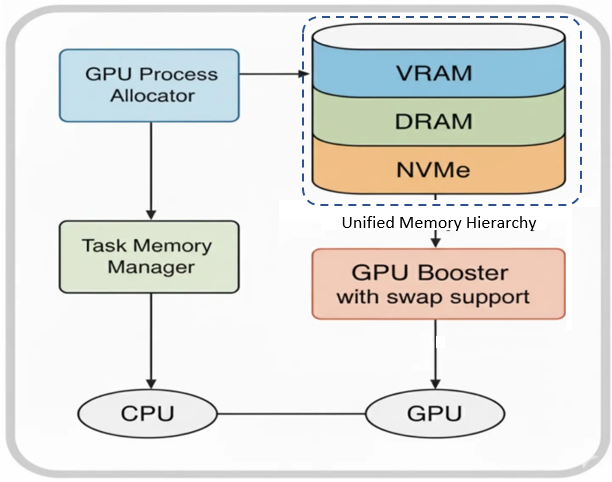
\includegraphics[width=0.95\linewidth]{figures/design.png}
\caption{System overview figure reproduced from the attached manuscript materials, illustrating the key modules used to coordinate hierarchical memory tiers during inference.}
\label{fig:orion_overview}
\end{figure}

